\chapter{Programmation non linéaire}
\label{chap:nonlinear}

Nous pouvons généraliser le programme linéaire introduit au chapitre précédent comme suit:
\begin{align*}
\max_x\ & f(x_1,\ldots,x_n) \\
\text{s.c.} & g_1(x_1,\ldots,x_n) \leq b_1, \\
& \vdots \\
& g_m(x_1,\ldots,x_n) \leq b_m.
\end{align*}
Si $f$ et $g_i$, $i = 1,\ldots,m$, sont linéaires, nous retrouvons le programme linéaire précédemment introduit, mais il n'existe pas de raison de se limiter à de tels cas.

En général, nous supposerons aussi que toutes ces fonctions sont deux fois dérivables.

\section{Fonctions convexes et concaves}

Soient $a$ et $b$ deux points dans $\RR^n$.
Le segment de droite joignant ces deux points est l'ensemble des points
\[
\lbrace x \in \RR^n \,|\, \exists\ \lambda \in [0,1] \mbox{ tel que } x = a + \lambda (b-a) = \lambda b +(1-\lambda)a \rbrace.
\]
Une fonction est {\sl convexe} si tout point sur le segment de droite joignant $f(a)$ et $f(b)$ se trouve au-dessus du graphe de $f$:
\begin{equation}
f(\lambda b +(1-\lambda)a) \leq \lambda f(b) + (1-\lambda)f(a),
\label{eq:convex_function}
\end{equation}
pour toute paire de points $(a,b)$.
Si cette inégalité est stricte, la fonction $f$ est dite {\sl strictement convexe}.
En remplaçant le sens de l'inégalité dans \eqref{eq:convex_function}, la fonction $f$ est dite {\sl concave}:
\[
f(\lambda b +(1-\lambda)a) \geq \lambda f(b) + (1-\lambda)f(a),
\]
pour toute paire $(a,b)$.
Si cette dernière inégalité est stricte, la fonction $f$ est {\sl strictement concave}.
La Figure~\ref{fig:convexity} illustre une fonction strictement convexe et une fonction strictement concave.

\begin{figure}[htb]
\begin{center}
\begin{tikzpicture}
\draw[->] (0,0) -- (5,0) node[below,right] {$x$};
\draw[->] (0,0) -- (0,5) node[above,left] {$f(x)$};
\draw (0,0) (-1,2) parabola bend (0.5,1) (4,4);
\draw (1.5,1) node [below]{fonction convexe};
\end{tikzpicture}
\begin{tikzpicture}
\draw[->] (0,0) -- (5,0) node[below,right] {$x$};
\draw[->] (0,0) -- (0,5) node[above,left] {$f(x)$};
\draw (0,0) (-1,2) parabola bend (2,4) (4,3);
\draw (2,4) node [above,sloped]{fonction concave};
\end{tikzpicture}
\end{center}
\caption{Fonctions convexe et concave}
\label{fig:convexity}
\end{figure}

\subsubsection{Tests de convexité et de concavité}

Supposons que $f$ est une fonction deux fois dérivable d'une seule variable. Alors,
\begin{enumerate}
\item
$f$ est convexe si et seulement si
\[
\forall\ x,\ \frac{d^2 f(x)}{dx^2} \geq 0;
\]
\item
$f$ est strictement convexe si
\[
\forall\ x,\ \frac{d^2 f(x)}{dx^2} > 0;
\]
\item
$f$ est concave si et seulement si
\[
\forall\ x,\ \frac{d^2 f(x)}{dx^2} \leq 0;
\]
\item
$f$ est strictement concave si
\[
\forall\ x,\ \frac{d^2 f(x)}{dx^2} < 0.
\]
\end{enumerate}

Supposons que $f$ est une fonction deux dérivable de deux variables.
Dans ce cas, nous utilisons la Table~\ref{tab:convexity} comme conditions nécessaires.
\begin{table}[htb]
\begin{tabular}{|c|c|c|c|c|}
\hline
& Convexe & Strict. convexe & Concave & Strict. concave \\
\hline
$\frac{\partial^2 f(x_1,x_2)}{\partial x_1^2}$ & $\geq 0$ & $> 0$ & $\leq 0$ & $< 0$ \\
\hline
$\frac{\partial^2 f(x_1,x_2)}{\partial x_2^2}$ & $\geq 0$ & $> 0$ & $\leq 0$ & $< 0$ \\
\hline
$\frac{\partial^2 f(x_1,x_2)}{\partial x_1^2}.\frac{\partial^2 f(x_2,x_2)}{\partial x_2^2}
- \left( \frac{\partial^2 f(x_1,x_2)}{\partial x_1x_2} \right)^2$ & $\geq 0$ & $> 0$ & $\geq 0$ & > 0 \\
\hline
\end{tabular}
\caption{Test de convexité et de concavité pour une fonction à deux variables deux fois dérivable}
\label{tab:convexity}
\end{table}

Ces tests se généralisent à des fonctions de plus de deux variables en utilisant le Hessien (la matrice des dérivées secondes).
Deux résultats supplémentaires sont utiles pour tester la convexité:
\begin{itemize}
\item
une fonction qui s'exprime comme la somme de fonctions convexes (concaves) est convexe (concave);
\item
l'opposé d'une fonction concave est convexe et vice-versa.
\end{itemize}

\subsection{Ensembles convexes}

Un ensemble est convexe si, pour toute paire de points de l'ensemble, le segment de droite joignant ces points est contenu dans l'ensemble.
Il est possible de démontrer qu'un ensemble est convexe grâce aux propriétés suivantes:
\begin{itemize}
	\item
	si $f$ est convexe, alors $\lbrace x \,|\, f(x) \leq b \rbrace$ est convexe;
	\item
	si $f$ est concave, alors $\lbrace x \,|\, f(x) \geq b \rbrace$ est convexe;
	\item
	l'intersection d'ensembles convexes est convexe.
\end{itemize}

\begin{example}[Wyndor Glass]
Modifions l'exemple Wyndor Glass en remplaçant certaines contraintes par une contrainte non linéaire.
\begin{align*}
\max z &= 3x_1 + 5x_2 \\
\st & x_1 \leq 4 \\
& 9x_1^2+5x_2^2 \leq 216 \\
& x_1 \geq 0,\ x_2 \geq 0.
\end{align*}
Le problème ainsi modifié peut se représenter comme sur la Figure~\ref{fig:wyndor_nonlinear}.
\begin{figure}[htbp]
\begin{center}
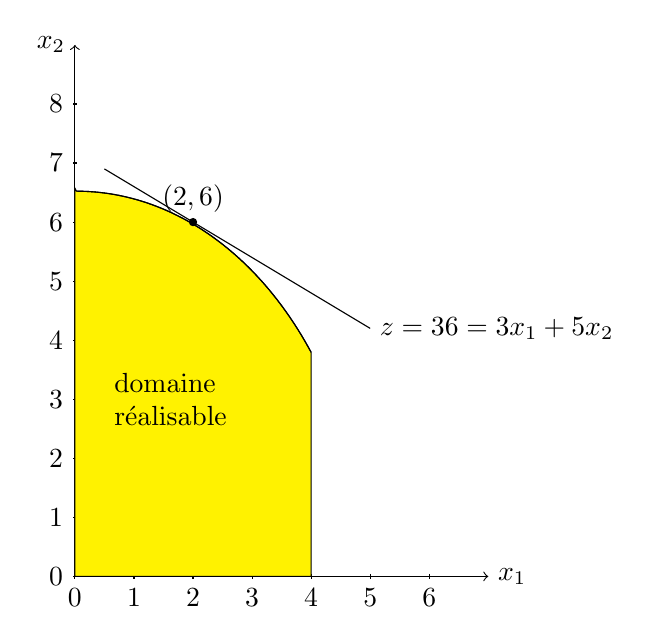
\begin{tikzpicture}[scale=0.75]
\draw[->] (0,0) -- (7,0) node[below,right] {$x_1$};
\draw[->] (0,0) -- (0,9) node[above,left] {$x_2$};
\draw (0.5,6.9) -- (5,4.2) node[right] {$z = 36 = 3x_1+5x_2$};

\foreach \x in {0,1,2,3,4,5,6}
  \draw (\x,1.2pt) -- (\x,-1pt) node[anchor=north] {$\x$};
\foreach \y in {0,1,2,3,4,5,6,7,8}
  \draw (1pt,\y) -- (-1pt,\y) node[anchor=east] {$\y$};

\filldraw[fill=yellow]
  (0,0) -- (4,0) -- (4,3.795) arc (35.8:90:4.899 and 6.573) -- (0,6.573) -- (0,0);

\draw (4,3.795) arc (35.8:90:4.899 and 6.573);
  
\draw (2,3) node[text width=2cm,text ragged] {domaine réalisable};

\draw (2,6) node[above] {$(2,6)$};
\fill (2,6) circle (2 pt);

\end{tikzpicture}
\end{center}
\caption{exemple Wyndor Glass}
\label{fig:wyndor_nonlinear}
\end{figure}
Remarquons que l'objectif est concave (car linéaire) et que le domaine réalisable est convexe: c'est un modèle de {\sl programmation convexe}.
Dans le cas présent, la solution optimale est sur la frontière du domaine réalisable, mais ne correspond pas à un coin (l'intersection de deux contraintes).

Modifions encore l'exemple Wyndor Glass, mais cette fois en remplaçant l'objectif lineaire par
une fonction non lineaire, comme illustré sur la Figure~\ref{fig:wyndor_nonlinear2}:
\begin{align*}
\max z\ &= 126x_1-9x_1^2+182x_2-13x_2^2 \\
& x_1 \leq 4 \\
& 2x_2 \leq 12 \\
& 3x_1 + 2x_2 \leq 18
\end{align*}
\begin{figure}[htbp]
\begin{center}
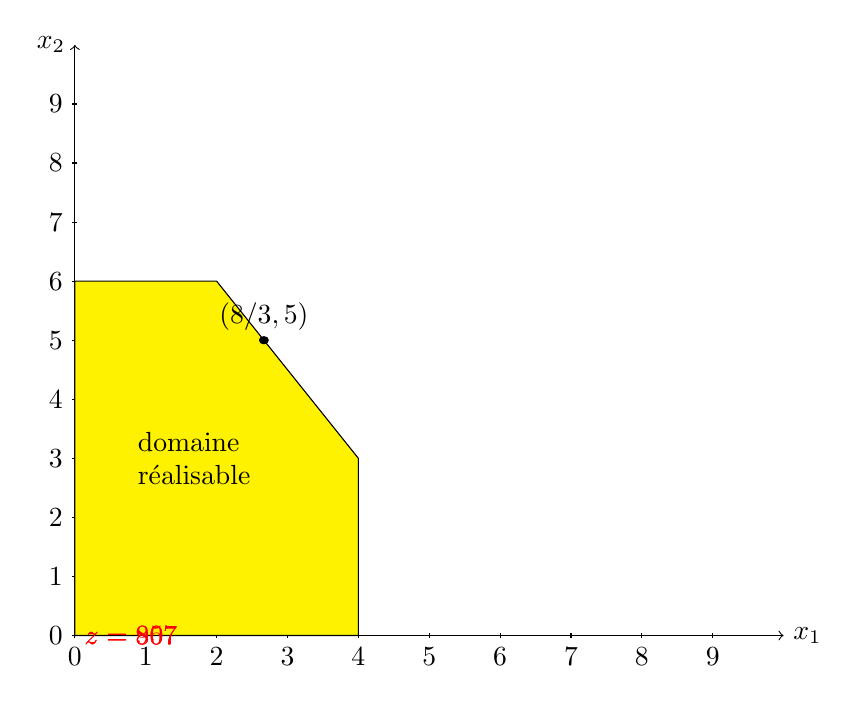
\begin{tikzpicture}[xscale=1.2,scale=0.75,samples=200]

\draw[->] (0,0) -- (10,0) node[below,right] {$x_1$};
\draw[->] (0,0) -- (0,10) node[above,left] {$x_2$};

\foreach \x in {0,1,2,3,4,5,6,7,8,9}
  \draw (\x,1pt) -- (\x,-1pt) node[anchor=north] {$\x$};
\foreach \y in {0,1,2,3,4,5,6,7,8,9}
  \draw (1pt,\y) -- (-1pt,\y) node[anchor=east] {$\y$};

\filldraw[fill=yellow]
  (0,0) -- (0,6) -- (2,6) -- (4,3) -- (4,0) -- (0,0);
  
\draw (2,3) node[text width=2cm,text ragged] {domaine réalisable};

\draw[color=red] plot[domain=2.65:7] function{7-sqrt(9*x/13.0*(14.0-x)-907.0/13.0+49)} node[right] {$z = 907$};
\draw[color=red] plot[domain=2.05:7] function{7-sqrt(9*x/13.0*(14.0-x)-857.0/13.0+49)}
node[right] {$z = 857$};
\draw[color=red] plot[domain=1.55:7] function{7-sqrt(x/13.0*(126-9*x)-807.0/13.0+49)}
node[right] {$z = 807$};

\draw (8.0/3,5) node[above] {$(8/3,5)$};
\fill (8.0/3,5) circle (2 pt);

\end{tikzpicture}
\end{center}
\caption{exemple Wyndor Glass - cas 2}
\label{fig:wyndor_nonlinear2}
\end{figure}

Nous pouvons à nouveau remarquer que l'objectif est concave et que le domaine réalisable est convexe: c'est aussi un modèle de programmation convexe.
Ici, la solution optimale $(8/3,5)$ est sur la frontière du domaine réalisable, mais ne correspond pas à un point extrême du domaine réalisable.

Considérons le même exemple, mais avec une fonction objectif différente, tel que représenté sur la Figure~\ref{fig:wyndor_nonlinear3}:
\begin{align*}
\max z\ &= 54x_1-9x_1^2+78x_2-13x_2^2 \\
& x_1 \leq 4 \\
& 2x_2 \leq 12 \\
& 3x_1 + 2x_2 \leq 18
\end{align*}
\begin{figure}[htbp]
\begin{center}
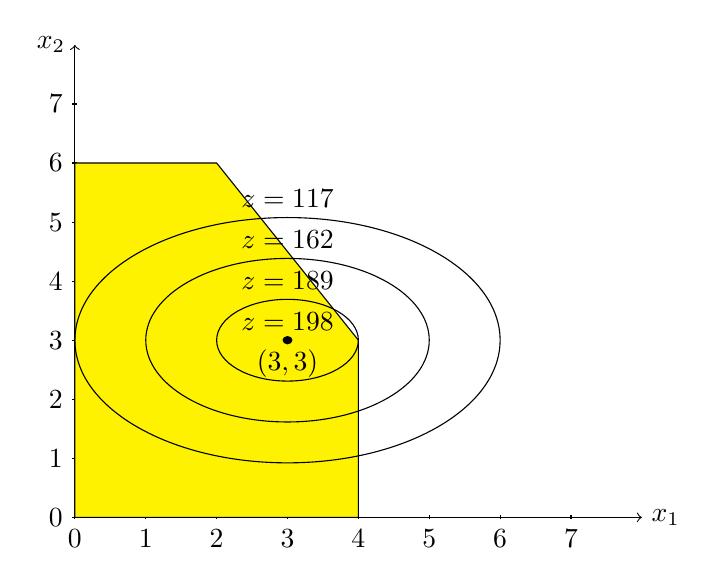
\begin{tikzpicture}[xscale=1.2,scale=0.75,samples=100]

\draw[->] (0,0) -- (8,0) node[below,right] {$x_1$};
\draw[->] (0,0) -- (0,8) node[above,left] {$x_2$};

\foreach \x in {0,1,2,3,4,5,6,7}
  \draw (\x,1pt) -- (\x,-1pt) node[anchor=north] {$\x$};
\foreach \y in {0,1,2,3,4,5,6,7}
  \draw (1pt,\y) -- (-1pt,\y) node[anchor=east] {$\y$};

\filldraw[fill=yellow]
  (0,0) -- (0,6) -- (2,6) -- (4,3) -- (4,0) -- (0,0);

\draw(3,3) ellipse (1 and 9.0/13.0);
\draw(3,3+9.0/13.0) node[above] {$z=189$};
\draw(3,3) ellipse (2 and 18.0/13.0);
\draw(3,3+18.0/13.0) node[above] {$z=162$};
\draw(3,3) ellipse (3 and 27.0/13.0);
\draw(3,3+27.0/13.0) node[above] {$z=117$};

\draw (3,3) node[above] {$z = 198$};
\draw (3,3) node[below] {$(3,3)$};
\fill (3,3) circle (2 pt);

\end{tikzpicture}
\end{center}
\caption{exemple Wyndor Glass - cas 3}
\label{fig:wyndor_nonlinear3}
\end{figure}
Il s'agit à nouveau d'un modèle de programmation convexe, avec comme solution optimale $(3,3)$, laquelle se trouve à l'intérieur du domaine réalisable.
La fonction objectif est la somme de deux fonctions d'une seule variable.
Si nous annulons les dérivées de chacune de ces fonctions, nous obtenons la solution unique $(3,3)$, qui se trouve à l'intérieur du domaine; c'est donc nécessairement la solution optimale.

Revenons sur la fonction objectif initiale, mais introduisons une contrainte non-linéaire, qui définit un domaine réalisable non-convexe, comme illustré sur la Figure~\ref{fig:wyndor_nonlinear4}:
\begin{align*}
\max z &= 3x_1 + 5x_2 \\
\st & x_1 \leq 4 \\
& x_2 \leq 7 \\
& 8x_1-x_1^2+14x_2-x_2^2 \leq 49 \\
& x_1 \geq 0,\ x_2 \geq 0.
\end{align*}
Le problème ainsi modifié peut se représenter comme sur la Figure~\ref{fig:wyndor_nonlinear4}.
\begin{figure}[htbp]
\begin{center}
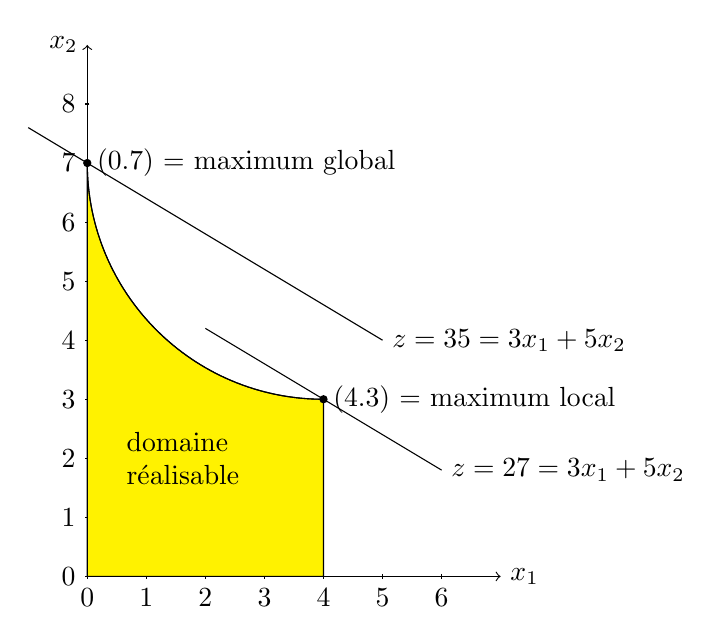
\begin{tikzpicture}[scale=0.75]
\draw[->] (0,0) -- (7,0) node[below,right] {$x_1$};
\draw[->] (0,0) -- (0,9) node[above,left] {$x_2$};

\foreach \x in {0,1,2,3,4,5,6}
  \draw (\x,1.2pt) -- (\x,-1pt) node[anchor=north] {$\x$};
\foreach \y in {0,1,2,3,4,5,6,7,8}
  \draw (1pt,\y) -- (-1pt,\y) node[anchor=east] {$\y$};

\filldraw[fill=yellow]
  (0,0) -- (4,0) -- (4,3) arc(270:180:4) -- (0,0);

\draw (4,3) arc(270:180:4);
  
\draw (2,2) node[text width=2cm,text ragged] {domaine réalisable};

\draw (-1,7.6) -- (5,4) node[right] {$z = 35 = 3x_1+5x_2$};
\draw (2,4.2) -- (6,1.8) node[right] {$z = 27 = 3x_1+5x_2$};

\draw (0,7) node[right] {$(0.7)$ = maximum global};
\fill (0,7) circle (2 pt);
\draw (4,3) node[right] {$(4.3)$ = maximum local};
\fill (4,3) circle (2 pt);

\end{tikzpicture}
\end{center}
\caption{exemple Wyndor Glass - cas 4}
\label{fig:wyndor_nonlinear4}
\end{figure}
Dans ce modèle de {\sl programmation non convexe}, nous remarquons la présence de deux maxima locaux:
\begin{itemize}
	\item
	$x$ est un {\sl maximum local} si $f(x) \geq f(a)$ pour tout $a$ réalisable suffisamment près de $a$;
	\item
	$(4,3)$ et $(0,7)$ sont des maxima locaux, mais $x^* = (0,7)$ est la {\sl maximum global}: $f(x) \geq f(a)$ pour tout $a$ réalisable.
\end{itemize}
Les méthodes classiques de programmation non-linéaire permettent d'identifier un maximum local, mais pas nécessairement le maximum global, alors qu'en programmation convexe, tout maximum local est global.
\end{example}

\section{Algorithmes}

\subsection{L'algorithme du simplexe dans le cas non-linéaire}

Le succès de l'algorithme du simplexe en programmation linéaire a naturellement motivé le développement de techniques similaires pour l'optimisation non-linéaire.
Une telle approche fut proposée en par Nelder et Mead~\cite{NeldMead65}.
Néanmoins, la notion de point extrême est beaucoup plus délicate à exploiter en non-linéaire, en particulier en l'absence de contraintes.
Il convient de construire un polyhèdre artificielle, ce qui n'est pas immédiat, et en pratique, la méthode souffre de l'absence de garantie de convergence, excepté pour des fonctions convexes à une variable~\citep{LagaReedWrigWrig98}.
Nous pouvons même observer une convergence vers un point non-stationnaire~\cite{McKi98}.
Un algorithme d'optimisation sans garantie de convergence est appelé {\sl heuristique}.s
Cette méthode est pourtant encore fréquemment employée, en particulier par les ingénieurs.
La fonction \verb|fminsearch| de Matlab~\footnote{Nous nous référons ici à la version 7.9, Release 2009b, mise en circulation le 4 septembre 2009.} implémente ainsi cet algorithme.
Malgré ce succès, aucun algorithme d'optimsation non-linéaire moderne ne se fonde sur le simplexe, et il convient dès lors d'éviter autant que possible de maintenir un tel usage.
De meilleurs résultats seront obtenus en employant des outils plus appropriés.

\subsection{Optimisation sans contrainte}

Considérons tout d'abord le cas d'un modèle de programmation non-linéaire dans lequel il n'y a aucune contrainte:
\[
\max f(x_1,x_2,\ldots,x_n).
\]
Il est alors possible de montrer que si $x^* = (x_1^*,x_2^*,\ldots,x_n^*)$ est un maximum local, alors
\[
\frac{\partial f(x^*)}{\partial x_j},\ j = 1,2,\ldots,n.
\]
En d'autres mots, lorsque la dérivée s'annule en un point donné, ce point {\sl peut être} un maximum local, mais l'inverse n'est pas nécessairement vérifié: ce point peut aussi être un minimum local ou un point de selle.
Par contre, si $f$ est concave, un point où la dérivée s'annule est nécessairement un maximum global.
De plus, si $f$ est strictement concave, un tel maximum global est unique.

Dans le cas d'une fonction non concave, afin de trouver un maximum global, il faut
\begin{itemize}
	\item
	identifier tous les maxima locaux;
	\item
	identifier celui de plus grande valeur;
	\item
	vérifier que la fonction est bornée supérieurement (sinon, il n'y a pas de maximum global). 
\end{itemize}
Le problème est qu'identifier tous les maxima locaux peut être extrêmement difficile.

\subsection{Méthode de la bissection}

Considérons en premier lieu le cas le plus simple: la fonction objectif $f$ est concave et comporte une seule variable.
Il est alors possible de montrer que, si $x^*$ est une solution optimale et il existe $x^i$ et $x^u$ tels que $x^i \leq x^* \leq x^u$ et $f(x^i) \ne f(x)$, $f(x^u) \ne f(x)$, alors il existe $a$ et $b$ tels que $a \leq x^* \leq b$ et
\begin{align*}
\frac{d f(x)}{dx} > 0,& \text{ si } x < a,\\
\frac{d f(x)}{dx} = 0,& \text{ si } x = x^*,\\
\frac{d f(x)}{dx} < 0,& \text{ si } x > b.\\
\end{align*}
Si $f$ est strictement concave en $x^*$, alors $a = x^* = b$, comme illustré sur la Figure~\ref{fig:concavity_maximum}.
\begin{figure}[htb]
\begin{center}
\begin{tikzpicture}
\draw[->] (0,0) -- (5,0) node[below,right] {$x$};
\draw[->] (0,0) -- (0,5) node[above,left] {$f(x)$};
\draw (0,0) (-1,-1) parabola bend (1.5,4) (4,-1);
\fill (1.5,4) circle (2 pt);
\draw (1.5,4) node[above] {$\frac{df(x)}{dx} = 0$};
\draw[help lines,color=blue] (1.5,4) -- (1.5,0) node[below] {$x^*$};
\end{tikzpicture}
\end{center}
\caption{Maximum d'une fonction strictement concave}
\label{fig:concavity_maximum}
\end{figure}
\begin{algo}{Méthode de la bissection}
\begin{enumerate}
	\item Nous fixons d'abord une borne inférieur $x^i$ pour laquelle la dérivée en ce point est strictement positive.
	\item Nous déterminons également une borne supérieure $x^u$ pour laquelle la dérivée en ce point est strictement négative.
	\item Si les deux bornes ne sont pas suffisamment près l'une de l'autre, i.e. la distance $x^u-x^i$ est trop grande, nous prenons le point milieu entre les deux bornes comme point candidat $x^c$:
	\[
	x^c = \frac{x^i+x^u}{2},
	\]
	et nous passons à l'étape suivante.
	Sinon, c'est-à-dire si
	\[
	x^u-x^i \leq 2\epsilon,
	\]
	avec $\epsilon > 0$ suffisamment petit,	nous nous arrêtons: $x^c$ est une approximation suffisamment précise de la solution optimale.
	\item
	Si la dérivée en $x^c$ est nulle, arrêt: $x^c$ est la solution optimale.
	\item
	Si la dérivée en $x^c$ est positive, nous posons $x^i = x^c$.
	\item
	Si la dérivée en $x^c$ est négative, nous posons $x^u = x^c$.
	\item Retour à l'étape 3.
\end{enumerate}
\end{algo}

\subsection{Méthode du gradient}

Considérons une fonction concave $f$ de {\sl plusieurs variables}. La méthode de la bissection ne peut plus s'appliquer, aussi nous devons nous tourner vers une meilleure alternative.
La gradient de $f$ au point $x'$ est défini comme
\[
\nabla_x f(x') = \begin{pmatrix}
\frac{\partial f(x)}{\partial x_1} \\
\frac{\partial f(x')}{\partial x_2} \\
\vdots \\
\frac{\partial f(x')}{\partial x_n} \\
\end{pmatrix}'.
\]
Il est possible de montrer que le gradient correspond a une direction d'augmentation de la valeur de $f$.
Ainsi, dans la méthode du gradient, nous nous déplaçons dans la direction du gradient en tentant d'augmenter au maximum la valeur de l'objectif.
A partir d'un point initial $x'$, nous effectuons un deplacement dans la direction du gradient vers un nouveau point $x$:
\[
x = x'+s,
\]
où $s = t^*\nabla_x f(x)$.
Dans cette formule, $t^*$ est la solution du problème de maximisation suivant:
\[
\max_{t \geq 0} f(x'+t\nabla_x f(x')).
\]
C'est un problème de maximisation d'une fonction concave d'une seule variable: nous pouvons par conséquent le résoudre, par exemple en employant la méthode de la bissection

Nous posons ensuite $x'=x$, et nous itérons ainsi jusqu'à ce que le gradient s'annule (ou presque).
Nous avons par conséquent l'algorithme suivant.
\begin{algo}{Méthode du gradient}
\begin{enumerate}
\item Déterminer une solution initiale $x_0$. Posons $k = 0$. Nous fixons également une constante $\epsilon > 0$ suffisamment petite.
\item Résoudre le problème suivant:
\begin{equation}
\max_{t \geq 0} f(x_k+t\nabla_x f(x_k)).
\label{eq:gradient_subproblem}
\end{equation}
\item
Soit $t^*$ la solution optimale de \eqref{eq:gradient_subproblem}. Posons
\[
x_{k+1} = x_k+t^* \nabla_x f(x_k),
\]
et incrémentons $k$.
\item
Si
\[
\left| \frac{\partial f(x_k)}{\partial x_j} \right| \leq \epsilon,\ j =1,2,\ldots,n,
\]
arrêt. Sinon, nous retournons en 2.
\end{enumerate}
\end{algo}

\subsection{Optimisation sous contraintes}

Dans le cas d'un modèle de programmation non-lineéire sans contrainte, nous avons vu la condition d'optimalité suivante: si $x^* = (x_1^*, x_2^*,\ldots, x_n^*)$ est un maximum local, alors
\[
\frac{\partial f(x^*)}{\partial x_j} = 0,\ j = 1,\ldots,n.
\]
Cette condition n'est plus valable lorsqu'il y a des contraintes, car une solution optimale peut se trouver sur la frontière du domaine réalisable

\begin{example}
Nous souhaitons résoudre le programme
\begin{align*}
\max_x\ & f(x) = 6-x-x^2 \\
\st\ & x \geq 0. 
\end{align*}
Il est facile de se convaincre (voir Figure~\ref{fig:concavity_positivity}) que la solution optimale est $x^* = 0$, pourtant
\[
\frac{df(0)}{dx} = -1 < 0.
\]
\begin{figure}[htb]
\begin{center}
\begin{tikzpicture}[scale=0.75, xscale=1.6]
\draw[->] (0,0) -- (5,0) node[below,right] {$x$};
\draw[->] (0,0) -- (0,8) node[above,left] {$f(x)$};
\foreach \x in {0,1,2,3,4}
  \draw (\x,1.2pt) -- (\x,-1pt) node[anchor=north] {$\x$};
\foreach \y in {0,1,2,3,4,5,6,7}
  \draw (1pt,\y) -- (-1pt,\y) node[anchor=east] {$\y$};

\draw plot[domain=0:2.1] function{6-x*(1+x)};
\fill (0,6) circle (2 pt);
\draw (0,6) node[above,right] {$\frac{df(x)}{dx} < 0$};
\end{tikzpicture}
\end{center}
\caption{Maximum d'une fonction concave sous contrainte de positivité}
\label{fig:concavity_positivity}
\end{figure}
\end{example}

\subsection{Conditions d'optimalité}

Avec une contrainte de la forme $x \geq 0$, les conditions d'optimalité s'énoncent ainsi: si $x^* = (x_1^*, x_2^*,\ldots, x_n^*)$ est un maximum local, alors
\[
\begin{cases}
\frac{\partial f(x^*)}{\partial x_j} = 0,& \mbox{ si } x_j^* > 0, \\
\frac{\partial f(x^*)}{\partial x_j} \leq 0,& \mbox{ si } x_j^* = 0. \\
\end{cases}
\]
Il est plus délicat de dériver les conditions dans le cas général, où nous avons également des contraintes sont de la forme:
\[
g_i(x_1,x_2,\ldots,x_n) \leq b_i,\ i = 1,2,\ldots,m.
\]
Elles s'expriment en fonction des {\sl multiplicateurs de Lagrange} $u_i$ associés à chaque contrainte.

\subsubsection{Conditions KKT (Karush-Kuhn-Tucker)}

Si $x^* = (x_1^*, x_2^*,\ldots, x_n^*)$ est un maximum local, alors il existe $m$ nombres $u_1, u_2,\ldots, u_m$ tels que
\begin{align*}
\frac{\partial f(x^*)}{\partial x_j} -\sum_{i=1}^m u_i \frac{\partial g_i(x^*)}{\partial x_j} \leq 0 \\
x_j^* \left( \frac{\partial f(x^*)}{\partial x_j} -\sum_{i=1}^m u_i \frac{\partial g_i(x^*)}{\partial x_j} \right) = 0 \\
g_i(x^*) - b_i \leq 0,\ i = 1,2,\ldots,m, \\
u_i \left( g_i(x^*) - b_i \right) = 0,\ i = 1,2,\ldots,m, \\
u_i \geq 0,\ i = 1,2,\ldots,m, 
\end{align*}

Les conditions KKT peuvent également s'exprimer en omettant les contraintes de non-négativité, lesquelles peuvent être réecrites sous la forme
\[
-x_i \leq 0,
\]
ou être tout simplement absentes.
La forme qui suit est par conséquent plus générale, et plus communément admise en programmation non-linéaire (voir par exemple Nocedal et Wright~\cite{NoceWrig99}).
Si $x^* = (x_1^*, x_2^*,\ldots, x_n^*)$ est un maximum local, alors il existe $m$ nombres $u_1, u_2,\ldots, u_m$ tels que
\begin{align*}
\frac{\partial f(x^*)}{\partial x_j} -\sum_{i=1}^m u_i \frac{\partial g_i(x^*)}{\partial x_j} = 0 \\
g_i(x^*) - b_i \leq 0,\ i = 1,2,\ldots,m, \\
u_i \left( g_i(x^*) - b_i \right) = 0,\ i = 1,2,\ldots,m, \\
u_i \geq 0,\ i = 1,2,\ldots,m, 
\end{align*}

\begin{example}[Conditions KKT]
Considérons le problème
\begin{align*}
\max\ & f(x_1,x_2) = \ln(x_1 +1) + x_2\\
\st & 2x_1 + x_2 \leq 3, \\
& x_1 \geq 0, x_2 \geq 0.
\end{align*}
Nous pouvons donc considérer qu'il n'y a qu'une seule contrainte avec
\[
g_1(x_1,x_2) = 2x_1 + x_2,
\]
et $b_1 = 3$.
Nous associons à cette contrainte un multiplicateur $u_1 \geq 0$.
Outre les contraintes de non-negativité, nous avons alors les conditions suivantes:
\begin{align*}
\frac{1}{x_1^*+1} - 2u_1 &\leq 0, \\
1-u_1 &\leq 0, \\
x_1^* \left( \frac{1}{x_1^*+1} - 2u_1 \right) &= 0, \\
x_2^*(1-u_1) &= 0, \\
2x_1^*+x_2^*-3 &\leq 0, \\
u_1(2x_1^*+x_2^*-3) &= 0.
\end{align*}
Nous obtenons $u_1 \geq 1$. Puisque $x_1^* \geq 0$, nous en déduisons
\[
\frac{1}{x_1^*+1} - 2u_1 < 0.
\]
Par conséquent, $x_1^* = 0$.
Puisque $u_1 \ne 0$, nous avons
\[
2x_1^* + x_2^* - 3 = 0,
\]
et par conséquent $x_2^* = 3$. Dès lors, $u_1 = 1$.
Les conditions KKT sont donc satisfaites en un seul point: $(0,3)$.
Il s'agit bien d'un maximum global, car la fonction objectif est concave et le domaine réalisable est convexe (modèle de programmation convexe).

En utilisant la version plus générale des conditions KKT, nous avons les conditions
\begin{align*}
\frac{1}{x_1^*+1} - 2u_1 + u_2 &\leq 0, \\
1-u_1 +u_3 &\leq 0, \\
2x_1^*+x_2^*-3 &\leq 0, \\
u_1(2x_1^*+x_2^*-3) &= 0, \\
-x_1 \leq 0,\\
-x_2 \leq 0,\\
u_2x_1 = 0,\\
u_3x_2 = 0.
\end{align*}
Il est facile de vérifier que la solution de ce système est
\[
x_1 = 0, x_2 = 3, u_1 = 1, u_2 = 1, u_3 = 0.
\]
\end{example}

\begin{small}
\section{Notes}

Ce chapitre se base en grande partie sur les notes de cours de Bernard Gendron, 2007.

\end{small}
